%Technology: precise description of the technology / approach that is used

% Inspiré de la section 10 du papier formose

To meet the \mpc, we have decided to use the general
approach of model federation~\cite{Golra2016-federation}. \emph{Model
  federation} is a way to assemble models using some kind of
low-coupling links. It has been studied to answer the OMG' RFP
Semantic Modeling for Information Federation (SIMF)~\cite{simf}. In
contrast to approaches that compose metamodels into a single large
metamodel grouping all needed entities, model federation build links
among models and metamodels (even through levels) to make ``things''
work together. As an illustration of this feature, we developed a
free-modeling editor -- freeing oneself from the bonds of
model/metamodel conformity -- that is presented
in~\cite{models2016-freemodel}. Another very interesting feature of
this approach is the strong decoupling among tools that remain usable
after federations are made.

We decided to use this approach since it offers the possibility to
link and to navigate among levels. Before we describe the overall
architecture in next section, here are some key concepts implemented
in the Openflexo~\cite{openflexo_link} framework.

% figure
% Dans la suite les références à la figure sont commentés

\begin{figure}[t]
    \centering
    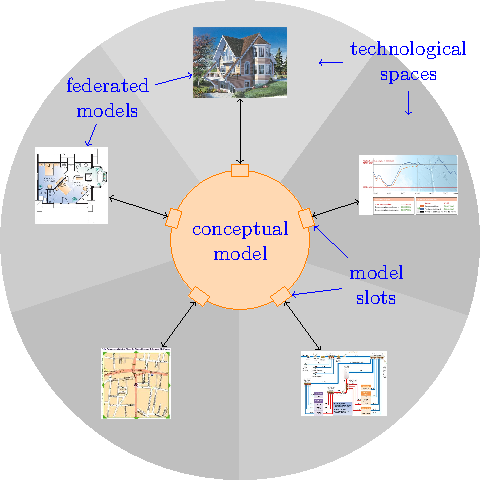
\includegraphics[width=\columnwidth]{Figures/federation.pdf}
    \caption{The model federation approach}
    \label{fig:mf}
\end{figure}

This framework relies on the architecture of Figure~\ref{fig:mf}. A federation
gathers a set of conceptual models, named \emph{virtual models} and a
set of \emph{federated models}. Each federated model pertains to a
\emph{technological space} and uses the language of its specific
paradigm while a virtual model is built using the Flexo Modeling
Language (FML). Each federated model can be viewed as an autonomous
component that may evolve with its own tooling. The virtual models
serve as control components.
In this paper, we mainly use the conceptual models and more precisely FML its domain specific modeling language. The only use of the federation aspect is on the tooling made for the process language.

\begin{figure}[t]
    \centering
    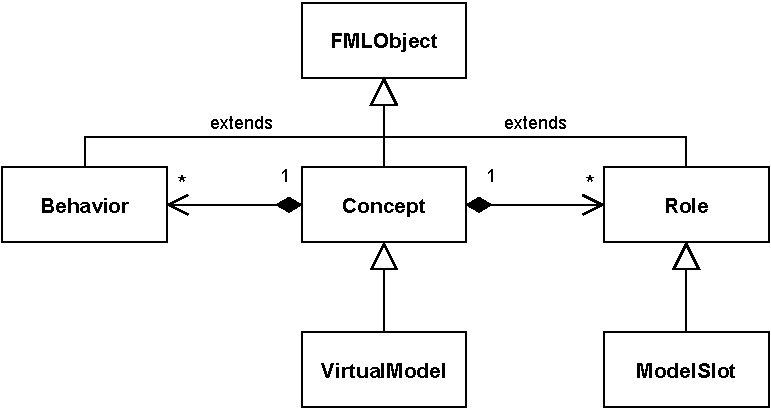
\includegraphics[width=\columnwidth]{Figures/FMLCoreModel.pdf}
    \caption{The FML core metamodel}
    \label{fig:mm}
\end{figure}
\noteAntoine{Dans la figure ne manque-t-il pas les containements ? (VM vers Concepts)}

FML simplified metamodel is provided in Figure~\ref{fig:mm}. It is designed to reify models as virtual models. A virtual model
is composed of a set of \emph{concepts}, while itself being a concept.
Hence, virtual models are structuring units while concepts are the
core entities. A concept has a set of \emph{roles} and
\emph{behaviors}. A parallel to object-oriented approach can be useful
to understand FML\footnote{Some aspects of FML do not exist in object oriented approach.}. A concept corresponds to a class, its roles to the
attributes of the class and its behaviors to the methods of the class.
These roles have types defining the kind of value the role will point
at runtime.
Whenever a type external to the federation space is used, one needs to use a \emph{model slot}. A model
slot is a mediation entity in charge of giving
access to external elements using
a \emph{technology adapter}\footnote{It is a reusable library that defines
connections between the FML execution engine and a particular
technological space.}.

FML is designed to define not only the structure of virtual models but
also to define the collection of actions an engineer can perform on
them. These actions are called \emph{behaviors} and can either be called (like usual methods) or triggered by events. The reactive behaviors are mainly useful when models have to be synchronised. We did not
exploit this possibility in the challenge.


When the FML execution engine runs a federation, it creates virtual
model instances containing concept instances. Some concept instances
are connected to external elements through model slot instances.


The tool support for model federation framework,
Openflexo\footnote{\url{https://github.com/openflexo-team}}, is
developed as an open source initiative. This tool offers a FML
execution engine with an interactive virtual model design environment.
It has been used in several case studies including model mapping,
multi-paradigm process modeling and enterprise architecting. It has
also been used to build a tool, the freemodeling editor that has been
used in industrial projects~\cite{models2016-freemodel}. As of today, this tool
offers some mature technology adapters (\emph{docx} and \emph{excel}
for documents, EMF and OWL for modeling languages, JDBC for databases,
REST and XMLRPC for external services and one for diagramming tools)
and other more rudimentary (pdf, HTTP, XML, etc.).

Finally, tools have their own model. We have taken advantage of
Openflexo features to build, in parallel with the models and virtual
models required by the challenge, a drawing tool that makes our
solution (partially) executable.
